%-------------------------------------------------------------------------------
% configuration
%-------------------------------------------------------------------------------
%
% \file        configuration.tex
% \library     Documents
% \author      Chris Ahlstrom
% \date        2021-01-18
% \update      2021-03-22
% \version     $Revision$
% \license     $XPC_GPL_LICENSE$
%
%     Provides the configuration information.
%
%-------------------------------------------------------------------------------

\section{Seq66 Configuration}
\label{sec:configuration}

   \textsl{Seq66} configuration has become a lot more elaborate.
   Fortunately, most of the configuration is well documented with-in the
   \textsl{Seq66} "man" page and in the configuration files themselves.
   Therefore, this new discussion will be less prolix than it was for
   \textsl{Sequencer64}.  Here are the topics to discuss:

   \begin{itemize}
      \item \textbf{Command-line Options}
      \item \textbf{'rc' File}
      \item \textbf{'usr' File}
      \item \textbf{'ctrl' File}
      \item \textbf{'mutes' File}
      \item \textbf{'drums' File}
      \item \textbf{'palette' File}
      \item \textbf{'playlist' File}
   \end{itemize}

   After the first run of \textsl{Seq66},
   it will generate a set of configration files in the default
   \textsl{configuration} directory, with names dependent on the version of
   \textsl{Seq66} being run:

   \begin{verbatim}
      /home/user/.config/seq66/qseq66.rc
      /home/user/.config/seq66/qseq66.usr
      /home/user/.config/seq66/qseq66.ctrl
      /home/user/.config/seq66/qseq66.mutes
      /home/user/.config/seq66/qseq66.drums
      /home/user/.config/seq66/qseq66.playlist
   \end{verbatim}

   The palette file is not automatically generated.  It can be saved from the
   \textbf{Edit / Preferences / Display} tab.

   For \textsl{Microsoft Windows}, the default base name of the files is
   \texttt{qpseq66}, and the default configuration directory is

   \begin{verbatim}
        C:/Users/user/AppData/Local/seq66/
   \end{verbatim}

   When running \textsl{Seq66} from the \textsl{Non Session Manager}
   (see \sectionref{sec:sessions}),
   the configuration directory is automatically set to something like

   \begin{verbatim}
      /home/user/NSM Sessions/MySession/seq66.nRSIQ/config
   \end{verbatim}

   There is no palette file by default, but the user can create one.
   The color palettes are discussed in \sectionref{sec:palettes}.

   These files contain the the data for remote MIDI control, computer keyboard
   control, MIDI clock, JACK transport, and a many other settings.

   \textsl{Seq66} \textsl{always} overwrites the most of these files upon
   exiting.  One must therefore quit \textsl{Seq66} before making
   manual modifications to these files.

   Some of the settings can be modified in the \textbf{Edit / Preferences}
   dialog, or overridden from the command line.

\subsection{Configuration File Commonalities}
\label{subsec:configuration_file_commonalities}

   All of the \textsl{Seq66} configuration files have the following in common:

   \begin{itemize}
      \item \textbf{[Seq66] Section}
      \item \textbf{[comments] Section}
      \item \textbf{Numeric Settings}
      \item \textbf{Boolean Settings}
      \item \textbf{Variables}
      \item \textbf{Stanzas}
   \end{itemize}

   Generally, each configuration file has its own specific set
   of sections, each section-name being enclosed in square brackets in a very
   strict format:  No spaces inside the square brackets.  Sections are looked up
   by this name, including the square brackets, and the name must be exact.

\subsubsection{[Seq66] Section}
\label{subsec:configuration_common_seq66_section}

   This section is generally just informational.  At a minimum, it holds two
   variables:

   \begin{itemize}
      \item \texttt{config-type}.  This value indicates the type of the file,
      such as "ctrl" or 'rc'.
      \item \texttt{version}.  This value indicates the version of the file.
      Currently, it is not used, but once \textsl{Seq66} solidifies,
      it can be used to make adjustments for changes in configuration when
      reading older versions of files.
   \end{itemize}

   This section may also contain additional "global"
   variables specific to a given \texttt{config-type}.

\subsubsection{[comments] Section}
\label{subsec:configuration_common_comments_section}

   This section is also informational, but the user can edit this section to
   include information describing the purpose of the file.  For example, a
   'ctrl' file for a \textsl{Novation Launchpad} might describe the purpose of
   this file.  The comments stop at the first blank (not even spaces) line.  To
   skip a line in the comment, put a single space character on the blank line.

\subsubsection{Numeric Settings}
\label{subsec:configuration_common_numeric_settings}

   Numeric settings consist of a line containing one or more numbers, usually
   preceded by an explanatory comment, and followed by a standard script
   comment.

   \begin{verbatim}
      3    # grid_style
   \end{verbatim}

\subsubsection{Boolean Settings}
\label{subsec:configuration_common_boolean_settings}

   Boolean settings are the same as numerical settings, but have only
   two values: "0" or "1".

   \begin{verbatim}
      0        # flag to record incoming data by channel
   \end{verbatim}

\subsubsection{Variables}
\label{subsec:configuration_common_variables}

   Variable are a new style of value setting, and can encompass not only
   booleans and numeric values, but string values, which may correspond to
   enumerated values in the source code.  These values are specified by a
   section-name plus variable-name pair.

   \begin{verbatim}
      [mute-group-flags]
      save-mutes-to = both
      . . .
   \end{verbatim}

   If the variable value is a string value, especially the name of the file or
   a directory, it must be surrounded with quotes, in case the path has spaces
   in it.

   Also note that there are still a lot of old-style variable specifications in
   place.  As time allows, they will be fixed, one-by-one, in a manner that
   does not break old configurations.

\subsubsection{Stanzas}
\label{subsec:configuration_common_stanzas}

   Please note that, as of version 0.92.0 of \textsl{Seq66}, we have
   streamlined the control-file stanza by eliminating the "enabled" and
   "channel" columns in a stanza, since they can be encoded in the event/status
   byte (e.g. 0x90) instead.  Older versions of the 'ctrl' file will be
   upgraded automatically.

   A stanza in a \textsl{Seq66} configuration file consists of some data at the
   beginning, a set of values bracketed by square brackets, and some optional
   data at the end.  The values inside the square brackets are numeric, and can
   be in decimal format, sometimes hexadecimal format, or in binary "0/1"
   format.

   \begin{verbatim}
      0 "1" [ 0 0x00 0 0 0 ] [ 0 0x00 0 0 0 ] [ 0 0x00 0 0 0 ]  # Loop 0
      1 "q" [ 0 0x00 0 0 0 ] [ 0 0x00 0 0 0 ] [ 0 0x00 0 0 0 ]  # Loop 1
      2 "a" [ 0 0x00 0 0 0 ] [ 0 0x00 0 0 0 ] [ 0 0x00 0 0 0 ]  # Loop 2
      3 "z" [ 0 0x00 0 0 0 ] [ 0 0x00 0 0 0 ] [ 0 0x00 0 0 0 ]  # Loop 3
      . . .
   \end{verbatim}

   See \sectionref{subsubsec:configuration_ctrl_loop_control}, which describes
   the details of this layout.

\subsection{Command Line}
\label{subsec:configuration_command_line}

   Command-line options are well-described in the \textsl{Seq66} "man" page.
   Here, we will present a brief note about each option, and, where applicable, a
   reference to the corresponding configuration file option.
   Here is the basic command line:

   \begin{verbatim}
       qseq66 [options list] [MIDI filename]
   \end{verbatim}

   \optionline{-h}{-{}-help}
      Display a list of all command-line options, then exit.

   \optionline{-v}{-{}-version}
      Display the program version, then exit.

   \optionline{-H}{-{}-home [directory]}
      Change the "home" configuration directory from \texttt{\$HOME.config/seq66}
      The configuration files are loaded from or saved to the specified directory.

   \optionline{-b}{-{}-bus [buss]}
      Modifies the output buss number on \textsl{all} tracks when a MIDI file is
      read.  Useful for testing or quick-and-dirty setup.

   \optionline{-q}{-{}-ppqn [ppqn]}
      Supports modifying the PPQN value of Seq66, which is
      defaults to a value of 192.  This setting
      is written into the MIDI file when it is saved.
      The PPQN value can range from 32 to 19200, or
      be set to 0 to use the PPQN from the loaded file.

      \configref{usr}{user-midi-settings}{midi\_ppqn}.

   \optionline{-L}{-{}-lash}
      If LASH support is compiled into the program, this option
      enables it.  Deprecated.
      See \texttt{usr: [user-session] session}.

      \configref{usr}{user-session}{session}

   \optionline{-m}{-{}-manual-ports}
      \textsl{Seq66} won't attach the system's existing ALSA or JACK MIDI ports.
      Instead, it will create is own set of \textsl{virtual}
      input and output busses/ports.  The default number of port is 1 for input,
      and 16 for output, but these values can be changed in the 'rc' file.

      \configref{rc}{manual-ports}{flag for manual/virtual ports}

   \optionline{-a}{-{}-auto-ports}
      \textsl{Seq66} will automatically attach to the system's existing
      ALSA/JACK ports.

      \configref{rc}{manual-ports}{flag for manual/virtual ports}

   \optionline{-r}{-{}-reveal-ports}
      \textsl{Seq66} will show the names of the ALSA/JACK ports that the system
      defines, rather than the names defined in the 'usr' configuration file.

   \optionline{-R}{-{}-hide-ports}
      \textsl{Seq66} will show the names of the ALSA port that the 'user'
      configuration file define, rather than the names defined by ALSA.

      \configref{rc}{reveal-ports}{flag for reveal ports}

      \configref{usr}{user-midi-bus-definitions}{number of user-defined busses}

   \optionline{-A}{-{}-alsa}
      \textsl{Seq66} will run with ALSA, even if JACK is running.
      This options is "sticky" (they are saved).

   \optionline{-t}{-{}-jack-midi}
      \textsl{Seq66} will run with JACK, which is the default is JACK is
      running.

      \configref{rc}{jack-transport}{with\_jack\_midi}

   \optionline{-s}{-{}-show-midi}
      Dumps incoming MIDI to the screen.

   \optionline{-p}{-{}-priority}
      Runs at higher priority with a FIFO scheduler.

%  \optionline{n/a}{-{}-pass-sysex}
%     Passes any incoming SYSEX messages to all outputs.
%	Not yet fully implemented.

   \optionline{-k}{-{}-show-keys}
      Prints pressed key value.

   \optionline{-K}{-{}-inverse}
      Changes the color palette for the sequence editor and performance editor
      piano rolls.  Also note that the palette is highly configurable.

      \configref{palette}{palette}{inverse}

   \optionline{-X}{-{}-playlist [filename]}
      This option loads the given file-name as a play-list file.
      See \sectionref{sec:playlist}.

      \configref{rc}{playlist}{name}

      \configref{playlist}{playlist}{full}

   \optionline{-j}{-{}-jack-transport}
      \textsl{Seq66} will sync to JACK transport.

      \configref{rc}{jack-transport}{with\_jack\_transport}

   \optionline{-J}{-{}-jack-master}
      \textsl{Seq66} will try to be JACK master.

      \configref{rc}{jack-transport}{with\_jack\_master}

   \optionline{-C}{-{}-jack-master-cond}
      JACK master will fail if there is already a master.

      \configref{rc}{jack-transport}{with\_jack\_cond}

   \optionline{-M}{-{}-jack-start-mode [x]}
      When \textsl{Seq66} is synced to JACK, the following play modes
      are available: 0 = live mode; and 1 = song mode, the default.

      \configref{rc}{jack-transport}{song\_start\_mode}

   \optionline{-U}{-{}-jack-session-uuid [uuid]}
      Set the UUID for the JACK session.

   \optionline{-u}{-{}-user-save}
      Save the 'usr' configuration file when exiting.
      Normally, it is saved only if not present in the configuration directory,
      so as not to get stuck with temporary settings such as the -{}-bus option.

      \configref{rc}{auto-option-save}{auto-save-options-on-exit}

   \optionline{-f}{-{}-rc filename}
      Use a different 'rc' configuration file.
      It must be a file in the user's \texttt{\$HOME/.config/seq66}
      directory or the directory specified by the \texttt{-{}-home} option.
      The \texttt{.rc} extension is added if necessary.

   \optionline{-F}{-{}-usr filename}
      Use a different 'usr' configuration file.  Similar to the \texttt{-{}-rc}
      option.

   \optionline{-c}{-{}-config basename}
      Use a different configuration file base name for the 'rc' and 'usr'
      files.  For example, one can specify a full configuration for "testing",
      for "jack", or for "alsa", to set up
      \texttt{testing.rc} and \texttt{testing.usr},
      \texttt{jack.rc} and \texttt{jack.usr},
      \texttt{alsa.rc} and \texttt{alsa.usr}.

   \optionline{-o}{-{}-option opvalue}
      Provides additional options, since the application is running out of
      single-character options.  The \texttt{opvalue} set supported is:
      \begin{itemize}
         \item \texttt{daemonize} and \texttt{no-daemonize}.
            \index{daemonize}
            Makes the \texttt{seq66cli} application fork to the background, or
            \index{no-daemonize}
            makes the \texttt{seq66cli} application
            run in the foreground so that console output can be seen.
         \item \texttt{log=filename.log}.
            \index{log}
            Reroutes standard error and standard
            output messages to the given log-file.  This file is located in
            the configuration directory.
            If this file is present, additional log information is appended.
            The default log-file name is specified in the
            \texttt{[user-options]} section of the 'usr' file.
         \item \texttt{sets=8x8}.
            \index{variset}
            This option, informally known as "variset", allow some changes in
            the set size and layout from the default 4x8 = 32 sets layout.
            Consider this option to be experimental. Expect problems.
            To save these options to the 'usr' file, add the
            \texttt{-{}-user-save} option to the command line.
            In that file, the options modified are \texttt{mainwnd\_rows} and
            \texttt{mainwnd\_cols}.
         \item \texttt{scale=WxH}.
            \index{scaling}
            This option scales the main window by the given factors,
            ranging from 0.75 to 3.0.
         \item \texttt{mutes=value}. Specifies the saving of mute-groups
            to the 'mutes' file, 'midi' file, or 'both' files.
         \item \texttt{virtual=o,i}. Set up the manual-ports option with 'o'
            output ports and 'i' input ports.
      \end{itemize}

      Many of the above options are including in the relevant configuration
      files.  We will point to them in the future.

\subsection{'rc' File}
\label{subsec:configuration_rc}

   \begin{verbatim}
      /home/user/.config/seq66/qseq66.rc
   \end{verbatim}

   The 'rc' configuration file has undergone a lot of changes, including
   off-loading the keyboard control, MIDI control, and mutes control sections
   into their own files, and adding a few "variable" settings.
   Rather than repeating information already present in the self-documenting
   'rc' file, we will summarize the settings and refer the reader to the sample
   files for more information.

   The 'rc' file adds these \texttt{[Seq66]} options to the common
   data for all configuration files:

   \begin{verbatim}
      verbose = false
      sets-mode = normal
      port-namng = short
   \end{verbatim}

   \texttt{verbose} is the same as the \texttt{-{}-verbose} command-line option,
   except that, if set to "true", it affects every invocation of \textsl{Seq66}.

   The \texttt{sets-mode} option determines if sets are muted when going to the
   next play-screen ('normal'), while 'autoarm' will automatically
   unmute the next set.  The 'additive' options keeps the previous
   set unmuted when moving to the next set.  These are options requested by
   users.

  The port-naming values are 'short' or 'long'.  The short style
  just shows the port number and short port name; the long style
  shows all the numbers and the long port name.

\subsubsection{'rc' File / MIDI Control}
\label{subsubsec:configuration_rc_midi_control}

   \index{[midi-control-file]}
   \textsl{Seq66} offloads MIDI control to a separate file.
   Move or create
   the \texttt{[midi-control]} section to a separate file in
   the \textsl{Seq66} configuration directory, and add the following
   snippet:

   \begin{verbatim}
      [midi-control-file]
      "qseq66.ctrl"          # contains a whole [midi-control] section
   \end{verbatim}

   As with the 'rc' file, the 'ctrl' file is rewritten upon exit.
   For the details of the 'ctrl' file, see
   \sectionref{subsec:configuration_ctrl}.

\subsubsection{'rc' File / Mute Groups}
\label{subsubsec:configuration_rc_mute_groups}

   \begin{verbatim}
      [midi-group-file]
      "qseq66.mutes"         # contains a whole [mute-groups] section
   \end{verbatim}

   The mutes-groups sections is written on exit dependent on the
   \texttt{save-mutes-to} option in the mute-groups file.

\subsubsection{'rc' File / Color Palette}
\label{subsubsec:configuration_rc_color_palette}

   \begin{verbatim}
      [palette-file]
      1       # palette_active
      "qseq66.palette"
   \end{verbatim}

   The only need for a palette file is when the user is not satisfied with the
   default palette for the patterns, inverse colors, or hatching for some pattern
   piano roll items.  There is a button to save the current/default palette for
   later modification in the \textbf{Edit / Preferences / Display} tab.

\subsubsection{'rc' File / Note Mapper}
\label{subsubsec:configuration_rc_note_mapper}

   \begin{verbatim}
      [note-mapper]
      1
      "GM_DD-11.drums"
   \end{verbatim}

   This file can be used transform the existing drum (non-transposable) tracks
   into another set of drum tracks.  A lot of work has been done in the past
   with non-General-MIDI instruments (particularly consumer instruments like the
   \textsl{Yamaha PSS-780} or \textsl{Yamaha DD-11}.
   This option is useful for transformation older MIDI files into GM format.
   For the usage of the note-mapper, see
   \figureref{fig:pattern_editor_oneshot_recording}, and the surrounding
   discussion.

\subsubsection{'rc' File / Port Map}
\label{subsubsec:configuration_rc_port_map}

   The 'rc' file also supports a port map, which maps I/O ports from a
   permanent buss number to the actual system buss number.
   The pattern is set to output to a specific buss number; this buss number is
   associated with a port name; this port name is looked up to see what
   system buss number is the one to be used.  When the system setup changes,
   the pattern does not need to changed; only the port mapping may need to be
   changed.  If the port map covers all I/O ports ever possible on a system, it
   will not need to be changed.  See \sectionref{sec:port_mapping}.

\subsubsection{'rc' File / MIDI-Clock Section}
\label{subsec:configuration_rc_midi_clock}

   \index{[midi-clock]}
   The MIDI Clock fields contain the clocking state from the last 
   time \textsl{Seq66} was run, and their status, and their names.
   Turn off the clock with a 0, or on
   with a 1 (which means to send
   \textbf{MIDI Song Position}, and
   \textbf{MIDI Continue} if
   starting after tick 0), or on with positioning with a 2, which sends
   \textbf{MIDI Start}
   and then begins clocking after the position reaches a modulo of the
   \textbf{Clock Start Modulo value)}.  Luckily, the user-interface makes it
   easy to select the desire value, and has tool-tips to instruct the user.
   This section has entries for each MIDI output buss.

   This configuration item is represented in the
   \textbf{Edit / Preferences / MIDI Clock} tab.

   \begin{verbatim}
      [midi-clock]
      5    # number of MIDI clocks (output busses)
      0 0    "[0] 14:0 Midi Through Port-0"
      1 0    "[1] 128:0 TiMidity port 0"
      2 0    "[2] 128:1 TiMidity port 1"
      . . .
   \end{verbatim}

\subsubsection{'rc' File / MIDI Clock Mod Ticks}
\label{subsubsec:configuration_rc_midi_cmt}

   \index{[midi-clock-mod-ticks]}
   This configuration item is the same as the
   \textbf{Edit / Preferences / MIDI Clock / Clock Start Modulo} option.

   \begin{verbatim}
      [midi-clock-mod-ticks]
      64
      0   # flag to record incoming data by channel
   \end{verbatim}

   The record-flag is kind of an outcast.  Not sure why it is here,
   something to rectify later.

\subsubsection{'rc' File / MIDI-Meta-Events Section}
\label{subsubsec:configuration_rc_midi_meta_events}

   \index{[midi-meta-events]}
   The new MIDI Meta events section is the start of additional options
   supporting meta events as normal events in \textsl{Seq66}.
   This section defines just one feature of MIDI meta-event handling at present.
   Normally, tempo events are supposed to occur in the first track (pattern 0).
   But one can move this track elsewhere to accomodate one's existing body of
   tunes.  If affects where tempo events are recorded.  The default value is 0,
   the maximum is 1023.  A pattern must exist at this number for it to work.
   \index{tempo-track-number}

   \begin{verbatim}
      [midi-meta-events]
      10      # tempo_track_number
   \end{verbatim}

   As per the MIDI specification, the first track (track 1 in track
   numbering, or pattern 0 in \textsl{Seq66} numbering) is \textsl{the}
   official track for certain MIDI meta events, such as
   \textbf{Set Tempo} and
   \textbf{Time Signature}.
   However, to accommodate existing tunes and their set
   arrangement, we allow the user to
   and change the tempo track to another pattern.

\subsubsection{'rc' File / Keyboard Control Section}
\label{subsubsec:configuration_rc_keyboard_control}

   The keyboard control section has been merged into the MIDI control section
   and been moved into the 'ctrl' file.
   There is no longer any user-interface to change the
   keyboard control, for two reasons:
   (1) It is pretty easy to read, understand, and edit the 'ctrl' file, and
   (2) There are many more controls in \textsl{seq66}, and creating a
   user-interface to edit them might not be worth the effort.
   We suspect most users will be happy enough with the default settings,
   and users of internationaly keyboards will find the 'ctrl' file easy enough
   to edit with a programmer's editor.
        
\subsubsection{'rc' File / JACK Transport}
\label{subsubsec:configuration_rc_jack_transport}

   This section holds the settings for both JACK transport and for native JACK
   MIDI mode.

   \index{[jack-transport]}
   The JACK Transport options are also command-line options.
   See \sectionref{subsec:configuration_command_line}.

   \begin{verbatim}
      [jack-transport]
      0   # with_jack_transport
      0   # with_jack_master
      0   # with_jack_master_cond
      0   # song_start_mode
      0   # with_jack_midi
   \end{verbatim}

   These options are described well in the 'rc' file.

   Please note that the JACK transport options are set to make sense, no
   matter what the user specifies.
   Also note that JACK transport is separately configurable from
   JACK MIDI, and each uses a different JACK client internally.
   We might combine them at some point, if necessary.

\subsubsection{'rc' File / MIDI Input}
\label{subsubsec:configuration_rc_midi_input}

   \index{[midi-input]}
   This configuration item is represented in the
   \textbf{MIDI Input} tab in the \textbf{Edit / Preferences}.
   The first number is a line count, and would equal the number of
   supported input ports.
   After that, this 'rc' entry here has two variables;
   the first is the port number,
   and the second number indicates whether it is disabled (0), or enabled (1).
   The next lines show the input busses present on the system (normally).

   \begin{verbatim}
      [midi-input]
      2   # number of MIDI busses
      0 1    "[0] 0:1 system:announce"
      1 0    "[1] 14:0 Midi Through Port-0"
   \end{verbatim}

   Again, see the 'rc' file itself for more information.

\subsubsection{'rc' File / Manual ALSA Ports}
\label{subsubsec:configuration_rc_manual_ports}

   The name of this setting is a bit of a misnomer in a couple of ways:

   \index{ports!virtual}
   \index{ports!manual}
   \begin{enumerate}
      \item It actually refers to the usage of \textsl{virtual} MIDI ports.
         These are ports that are set up by the application so that other
         devices, applications, or session managers can connect
         \textsl{manually} to the MIDI application.
      \item This option is not just for ALSA.  It can also be used when
         running in native JACK mode, to support
         virtual JACK ports that can be connected manually (e.g. in the
         \textsl{QJackCtl} application.)
   \end{enumerate}

   \index{[manual-ports]}
   \begin{verbatim}
      [manual-ports]
      0   # flag for manual (virtual) ALSA or JACK ports
      8   # number of manual/virtual output ports
      4   # number of manual/virtual input ports
   \end{verbatim}

   \index{--auto-ports}
   The opposite of \texttt{-{}-manual-ports} is \texttt{-{}-auto-ports},
   which is the normal mode of running \textsl{Seq66}.
   In this mode, system MIDI input/output devices are discovered and
   automatically connected.

   It will create port names as per the settings in the 'usr' configuration
   file's sections:

   \begin{verbatim}
      [user-midi-bus-definitions]
      [user-midi-bus-N]
   \end{verbatim}

   These definitions can be used by JACK for connection, and these
   definitions can be used to specifically rename the ports that exist in the
   system.
   This option is misleading if one wants to have access to the
   actual ALSA/JACK ports that exist on the system.
   The next option gets around that issue.

\subsubsection{'rc' File / Reveal ALSA Ports}
\label{subsubsec:configuration_rc_reveal_ports}

   This option applies to both ALSA and JACK.

   \index{[reveal-ports]}
   \begin{verbatim}
      [reveal-ports]
      1   # flag for reveal ALSA ports
   \end{verbatim}

   \index{jack!reveal-ports}
   Turning on the reveal-ports option is necessary if one
   wants to see the actual port names defined by the system.
   It ignores the settings in the 'usr' configuration file's
   \texttt{user-midi-bus-definitions} and \texttt{user-midi-bus-N} sections.
   If this option is turned on, the definitions in the
   'usr' configuration file are \textsl{not} read from that file.

\subsubsection{'rc' File / Interaction Method}
\label{subsubsec:configuration_rc_interaction}

   \begin{verbatim}
      1   # allow_mod4_mode
      1   # allow_snap_split
      1   # allow_click_edit
   \end{verbatim}

   The \texttt{Mod4} ("Windows" key) option is still available, but no longer
   necessary.  Also removed is the option for the "fruity" option
   of \textsl{Seq24}.
   It will be added if there is a clamor for it.

   \index{[allow-snap-split]}
   \index{new!snap-split}
   This option comes from the \textsl{seq32} project.  It allows for
   pattern-splitting in the Song editor at snap points, rather than just
   at the middle of the pattern.

   \index{[allow-click-edit]}
   \index{new!click-edit}
   This option allows one to enable/disable the ability to double-click
   in a pattern slot in the main window to bring it up for editing.
   This can interfere with a live performance where muting/unmuting come fast
   enough to be seen as a double-click.

\subsubsection{'rc' File / Auto Option Save}
\label{subsubsec:configuration_rc_auto_option_save}

   \index{[auto-option-save]}
   This item determines if the 'rc' configuration file (and other files)
   is saved upon exit of \textsl{Seq66}.
   The normal behavior is to save it,
   which can sometimes be inconvenient when one is just trying out some
   command-line options.

   \begin{verbatim}
      [auto-option-save]
      0     # auto-save-options-on-exit support flag
   \end{verbatim}

\subsubsection{'rc' File / Last Used Directory}
\label{subsubsec:configuration_rc_last_used_dir}

   The following item refers to the last directory in which one opened or
   saved a MIDI file.

   \index{[last-used-dir]}
   \begin{verbatim}
      [last-used-dir]
      /home/ahlstrom/Home/ca/mls/git/seq66/contrib/midi/
   \end{verbatim}

\subsubsection{'rc' File / Recent Files}
\label{subsubsec:configuration_rc_recent_files}

   The following item preserves a list of the last few MIDI files loaded.
   It is not filled when a MIDI file is loaded via a play-list.
   The first number is the count of recent-files.
   The second number is a boolean, set to "1" if the most-recent file
   should be loaded when \textsl{Seq66} starts.
   This option is useful as part of restoring a session.

   \index{[recent-files]}
   \begin{verbatim}
      [recent-files]
      2 1
      "/home/user/Home/ca/mls/git/seq66-alternate/contrib/midi/2Bars.midi"
      "contrib/midi/b4uacuse-seq24.midi"
   \end{verbatim}

\subsubsection{'rc' File / Play-List}
\label{subsubsec:configuration_rc_playlist}

   This item provides a configured set of named play-lists in a play-list file,
   and a flag to activate it.
   Having a playlist makes it easy to load song after song from pre-determined
   lists.
   
   \index{[playlist]}
   \begin{verbatim}
      [playlist]
      0     # playlist_active, 1 = active, 0 = do not use it
      "/home/ahlstrom/.config/seq66/sample.playlist"
   \end{verbatim}

   See \sectionref{sec:playlist}.
   It describes the setup, layout, and usage of a
   \textsl{Seq66} playlist file containing one or more playlists.

\subsection{'usr' File}
\label{subsec:configuration_usr}

   This section describes the \textsl{Seq66} 'usr' (or "user") file.
   The \textsl{Seq66} 'usr'
   configuration file provides a way to give more
   informative names to the MIDI busses, MIDI channels, and MIDI controllers of
   a given system setup, and allows for some tweaking of the application.
   This configuration overrides the default values
   of the \textbf{Event} drop-down list and menu items in the Pattern editor,
   and make them reflect the names of the MIDI Control (CC) values of one's
   devices.

   In \textsl{Seq66} it, also includes some items that affect the
   user-interface's look, and many other new configuration items.
%  At some point we will likely split this file into another configuration file
%  ("qseq66.ui"?)

   \index{usr!-u}
   \index{usr!--user-save}
   Unlike the 'rc' file, the 'usr' file is \textsl{not} written every time
   \textsl{Seq66} exits.  If the 'usr' files does not exist, one is
   created, but it is normally not overwritten thereafter.  To
   cause it to be overwritten at exit, run \textsl{Seq66} with the
   \texttt{-u} or \texttt{-{}-user-save} option:

   \begin{verbatim}
      $ qseq66 --user-save
   \end{verbatim}

   This option is recommended when one installs a new version of
   \textsl{Seq66}, which might add new options to the 'usr' file.
   One usually must edit the 'usr' file manually.
   There are a few items that can be tweaked in the \textsl{Seq66} application,
   and if they are modified, the user-save flag is turned on.

   By default, the list of MIDI devices that \textsl{Seq66} shows depends
   on one's system setup and whether the manual-port option is specified
   or not.  Here's our system, with the
   the \texttt{[manual-port]} option turned off, shown in a
   composite view with all menus one can look at for MIDI settings:

\begin{figure}[H]
   \centering 
   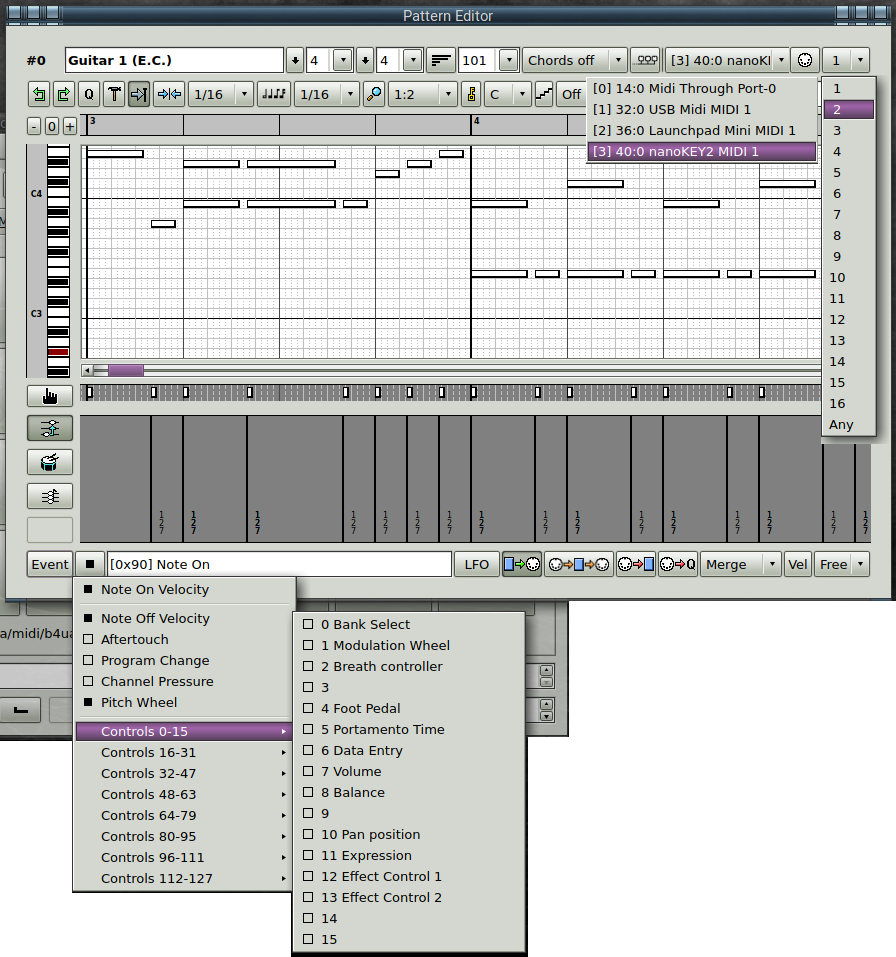
\includegraphics[scale=0.75]{configuration/usr/default-event-bus-channel-menus.png}
   \caption{Seq66 Composite View of Native Devices}
   \label{fig:default_event_bus_channel_menus}
\end{figure}

   at the top, the buss dropdown menu contains the MIDI busses/ports
   active on this computer.  At right, the MIDI channel shows
   the channels numbers that can be picked for buss 0.  At bottom left, we see
   the default controller values that \textsl{Seq66} includes.  We have
   no idea if these correspond to any controllers that the selected MIDI buss
   supports.  We \textsl{can} use this dropdown to see if any such controller
   events are in the loaded MIDI file, of course; a solid black square
   indicates that such an event was found in the pattern.

   to change the defaults, we can create a 'usr' file to set them up.
   the discussion here relies on the reader opening the file
   \texttt{sample.usr}, which is included in the shared \texttt{data/samples}
   directory provided once \textsl{Seq66} is installed.

   assume we have 3 MIDI "buss" devices hooked to our system:
   two Model "2x2" MIDI port devices, and an old PCR-30 MIDI controller
   keyboard.  Let's number them:

   \begin{enumerate}
      \item Model 2x2 A
      \item Model 2x2 B
      \item PCR-30
   \end{enumerate}

   then assume that we have nine different MIDI instruments in our kit.
   let's number them, too:

   \begin{enumerate}
      \item Waldorf Micro Q
      \item SuperNova
      \item DrumStation
      \item TX81Z
      \item WaveStation
      \item ESI-2000
      \item ES-1
      \item ER-1
      \item TB-303
   \end{enumerate}

   The \textsl{Waldorf Micro Q},
   the \textsl{SuperNova},
   and the \textsl{DrumStation} all have a large
   number of special MIDI controller values for modifying the sound they
   produce.
   The \textsl{DrumStation} accepts MIDI controllers that change various
   features of the sound of each type of drum it supports.

   The buss devices can be configured to route certain
   MIDI channels to certain MIDI devices.  Assume we have them
   set up this way:

   \begin{enumerate}
      \item Bus 0: Model 2x2 A
      \begin{itemize}
         \item SuperNova: channels 1 to 8
         \item TX81Z: channels 9 to 11
         \item Waldorf Micro Q: channels 12 to 15
         \item DrumStation: channel 16
      \end{itemize}
      \item Bus 1: Model 2x2 B
      \begin{itemize}
         \item WaveStation: channels 1 to 4
         \item ESI-2000: channels 5 to 14
         \item ES-1: channel 15
         \item ER-1: channel 16
      \end{itemize}
      \item Bus 2: PCR-30
      \begin{itemize}
         \item TB-303: channel 1
      \end{itemize}
   \end{enumerate}

   We use the \textbf{'usr' configuration file}.
   to show these items with the proper
   names associated with each device, channel, and controller value

   \index{seq66.usr}
   The \textsl{Seq24} configuration file was called
   \texttt{.seq24usr}, and it was stored in the user's \texttt{\$HOME}
   directory.
   \textsl{Seq66} uses a new file-name
   to take its place.
   After one runs \textsl{Seq66} for the first time (or after deleting
   the configuration files), it will generate a
   \texttt{seq66.usr} file in one's HOME directory:

   \begin{verbatim}
      /home/user/.config/seq66/seq66.usr
   \end{verbatim}

   It allows you to give an alias to 
   each MIDI bus, MIDI channel, and MIDI control 
   codes, per channel.
   The process for setting up the 'usr' file is to:

   \begin{enumber}
      \item Define one or more MIDI busses, the name of each, and what
         instruments are on which channels.  Each buss is configured in a
         section of the form "\texttt{[user-midi-bus-X]}", where "X" ranges
         from 0 on up.  Each buss then defines up to 16 channel entries.
         Each entry includes the channel number and the number of a
         section in the user-instrument section described next.
      \item Define all of the instruments and their controller
         names, if they have them.  Each instrument is configured in a
         section of the form "\texttt{[user-instrument-X]}", where "X"
         ranges from 0 on up.  Up to 128 controllers can be defined.
   \end{enumber}

   Let's walk through the structure of this setup, since it is a little bit
   tricky.

   The first important section in the 'usr' file
   is \texttt{[user-midi-bus-definitions]}.
   This section contains an number
   of \texttt{[user-midi-bus-N]} sections, where "N" ranges from 0 on upward.
   These correspond to the MIDI \textsl{output}
   busses expected to be in the system (ignoring the ALSA "announce" buss if
   ALSA is the MIDI engine being used).

   Each of the busses contains 16 (0 to 15) channel entries.
   These channels are referred to as "instrument numbers", and are
   represented as and linked to "instruments" in this section:

   \begin{verbatim}
      [user-instrument-definitions]
   \end{verbatim}

   Each instrument contains up
   to 128 controller values; these controller values are available in the
   \textbf{Event} button in the Pattern Editor, and their names are shown.

   So, each instrument is setup as a "channel" in a particular "buss".
   In the Pattern Editor, when a particular buss and channel is selected,
   the \textbf{Event} menu entries should match the controller entries set up
   in the 'usr' file.

   The list of devices and channels shown earlier
   can be seen in the \textsl{Seq66} sample file
   \texttt{sample.usr}.
   Deducting 1 from each device number and channel number (so that numbering
   starts from 0), and consulting the device manuals to determine the
   controller values supported, one can assemble a 'usr' configuration file
   that makes the setup visible in \textsl{Seq66}.

   Peruse the next couple of sections to understand a bit about the format of
   this file, following along in the sample 'usr' file.

\subsubsection{'usr' File / MIDI Bus Definitions}
\label{subsubsec:usr_file_midi_bus_definitions}

   \index{usr!user-midi-bus-definitions}
   \index{[user-midi-bus-definitions]}
   This section begins with an
   "INI" group marker \texttt{[user-midi-bus-definitions]}.
   It defines the number of user busses that will be configured in this file.

   \begin{verbatim}
      [user-midi-bus-definitions]
      3     # number of user-defined MIDI busses
   \end{verbatim}

   \index{usr!user-midi-bus-n}
   \index{[user-midi-bus-n]}
   This means that the 'usr' file will have three MIDI buss
   sections: [user-midi-bus-0], [user-midi-bus-1], and [user-midi-bus-2].
   Here's is an example of one such section:

   \begin{verbatim}
      [user-midi-bus-0]
      2x2 A (SuperNova,Q,TX81Z,DrumStation)
      16
      0 1
      1 1      # Instrument #1 of the [user-instrument-definitions] section
      . . .
      8 3      # Instrument #3 of the [user-instrument-definitions] section
      9 3
      . . .
      11 0     # Instrument #0 of the [user-instrument-definitions] section
      12 0     # This is the Waldorf Micro Q device
      . . .
      15 2     # Instrument #2 of the [user-instrument-definitions] section
   \end{verbatim}

   These instrument-definition
   sections are read from the 'usr' configuration file only if
   the "reveal ports" option is \textsl{off} ("0");
   this option can also be specified in the
   \texttt{[reveal-ports]} section of the 'rc' file.
   Otherwise, the actual port names reported by ALSA/JACK are shown.

   The \texttt{user-midi-bus-definitions} and \texttt{user-midi-bus-N} sections
   can be misleading if one wants to have access to the
   actual MIDI port names that exist on the system.
   It is left as an exercise for the reader to try these different combinations
   of show-port options.  Or one can consult the \textsl{Sequencer64 User
   Manual} to see the figures.

   \begin{itemize}
      \item Clocks View, -m (-{}-manual-ports)
      \item Inputs View, -m (-{}-manual-ports)
      \item Clocks View, -m (-{}-manual-ports) and -R (-{}-hide-ports)
      \item Clocks View, -r (-{}-reveal-ports)
      \item Inputs View, -r (-{}-reveal-ports)
      \item Clocks View, -R (-{}-hide-ports)
   \end{itemize}

\subsubsection{'usr' File / MIDI Instrument Definitions}
\label{subsubsec:usr_file_midi_instrument_definitions}

   \index{usr!user-instrument-definitions}
   \index{[user-instrument-definitions]}
   This section begins with an
   "INI" group marker \texttt{[user-instrument-definitions]}.
   It defines the number of user instruments that will be configured in this
   file.  This section defines characteristics, such as
   the meanings of MIDI controller values, of the instruments themselves,
   not the MIDI busses to which they attached.

   \begin{verbatim}
      [user-instrument-definitions]
      9     # number of user instrument
   \end{verbatim}

   \index{usr!user-instrument-n}
   \index{[user-instrument-n]}
   So this 'usr' file will define 9 instruments.  We provide only one section
   as an example.  Note that items without text default to the values
   prescribed by the General MIDI (GM) specification.

   \begin{verbatim}
      [user-instrument-0]
      Waldorf Micro Q                     # name of instrument
      128                                 # number of MIDI controllers
      0                                   # first controller value, unnamed
      1 Modulation Wheel
      2 Breath Control
      3 
      4 Foot Control
         . . .
      123 All Notes Off (0)
      124                                 # defaults to GM
      125 Unsupported
      126 Unsupported
      127                                 # defaults to GM
   \end{verbatim}

   Note the unnamed control numbers above.
   An unnamed control number might be an unsupported control number.
   It is termed to be "inactive".  In this case, the \textbf{Event} menu of
   the Pattern editor will show the default name of this controller.
   Again, though, the function denoted by this name might not be supported by
   the device.  In that case, it might be better to call it "Unsupported".
   See the examples above.  See the figure below for one example as set up using
   the \texttt{sample.usr} file:


\begin{figure}[H]
   \centering 
   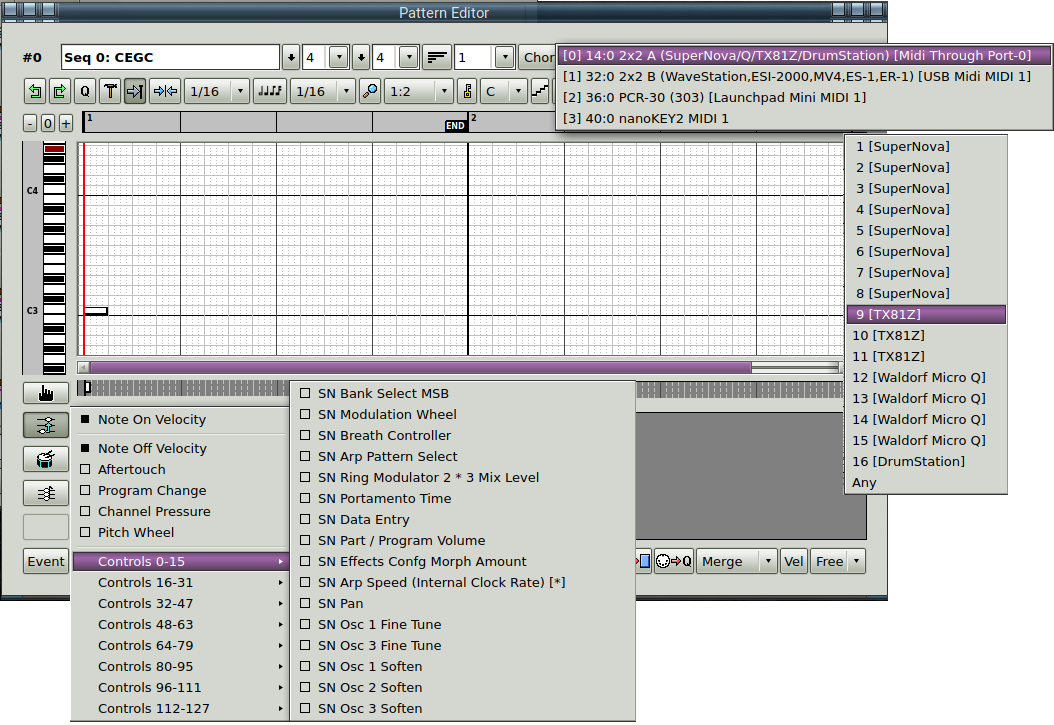
\includegraphics[scale=0.65]{configuration/usr/sample-usr-event-bus-channel-menus.png}
   \caption{Seq66 Composite View of Devices As Set in "sample.usr"}
   \label{fig:sample_usr_event_bus_channel_menus}
\end{figure}

\subsubsection{'usr' File / User Interface Settings}
\label{subsubsec:usr_file_user_interface_settings}

   \index{usr!user-interface-settings}
   \index{[user-interface-settings]}
   This section, new to \textsl{Seq66}, begins with an
   "INI" group marker \texttt{[user-interface-settings]}.

   It provides for a feature we will hopefully be able to complete some day:
   the complete specificition of the appearance of the user-interface.
   There is plenty of room to change the appearance of
   \textsl{Seq66} already!  Please try the settings and see what looks good.
   Refer to either the sample file or the file generated when \textsl{Seq66}
   first runs.

   \index{usr!grid-style}
   \index{usr!grid-brackets}
   \index{usr!mainwnd-rows}
   \index{usr!mainwnd-cols}
   \index{variset}
   \index{usr!max-sets}
   \begin{verbatim}
      [user-interface-settings]
      1       # grid_style
      2       # grid_brackets
      4       # mainwnd_rows
      8       # mainwnd_cols
      32      # max_sets
   \end{verbatim}

   There are a number of additional user-interface options.  See the generated
   or sample 'usr' file for descriptions.  Also see the chapter on palettes.

\subsubsection{'usr' File / User MIDI Settings}
\label{subsubsec:usr_file_user_midi_settings}

   \index{[user-midi-settings]}
   This section begins with an
   "INI" group marker \texttt{[user-midi-settings]}.
   It supports files with different PPQN, and and allows one to specify the
   global defaults for tempo, beats per measure, and so on.

   \index{usr!midi-ppqn}
   \index{usr!midi-beats-per-measure}
   \index{usr!midi-beats-per-minute}
   \index{usr!midi-beat-width}
   \index{usr!midi-buss-override}
   \index{usr!velocity-override}
   \begin{verbatim}
      [user-midi-settings]
      192    # midi_ppqn
      4      # midi_beats_per_measure/bar
      120    # midi_beats_per_minute
      4      # midi_beat_width
      -1     # midi_buss_override
      80     # velocity_override (-1 = 'Free')
   \end{verbatim}

   The \texttt{velocity-override} option fixes a long standing (from
   \textsl{Seq24}) bug where the actual incoming note velocity was always
   replaced by a hard-wired value.

   \index{usr!bpm-precision}
   \index{usr!bpm-step-increment}
   \index{usr!bpm-page-increment}
   \begin{verbatim}
      1      # bpm_precision
      0.1    # bpm_step_increment
      5.0    # bpm_page_increment
   \end{verbatim}

   The \texttt{bpm-precision}, \texttt{bpm-step-increment}, and
   \texttt{bpm-page-increment} values allow more precise control over tempo,
   which makes it easier to match the tempo of external music sources.  Note
   that the step-increment is used by the up/down arrow buttons, the up/down
   arrow keys, and the MIDI BPM control values.  The page-increment is used
   if the BPM field has focus and the Page-Up/Page-Down keys are pressed,
   and new MIDI control values have been added to support coarse MIDI
   control of tempo.

   \index{usr!midi-bpm-minimum}
   \index{usr!midi-bpm-maximum}
   \begin{verbatim}
      0       # midi_bpm_minimum
      360     # midi_bpm_maximum
   \end{verbatim}

   The \texttt{midi-bpm-minimum} and \texttt{midi-bpm-maximum} settings
   are used in scaling the display of Tempo events.
   By adjusting these values, one can more easily see the variations in
   tempo.  In a main window pattern slot, or in the song editor tempo track,
   this range is scaled to the full range of note values, 0 to 127.
   Generally, one wants to select a range that keeps the main tempo line at
   the middle height of the pattern display.

   To obtain these new settings, remember to backup the existing
   \textsl{seq66.usr}, then run \textsl{Seq66} with the
   \texttt{-{}-user-save} option, and then do a "diff" on the new file and the
   original to merge any old values that need to be preserved.  Then make any
   further tweaks to the new values.

\subsubsection{'usr' File / User Options}
\label{subsubsec:usr_file_user_options}

   \index{[user-options]}
   This section begins with an
   "INI" group marker \texttt{[user-options]}.
   It provides for additional options keyed by the
   \texttt{-o}/\texttt{-{}-option} options.
   This group of options serves to expand the options that are available, since
   \textsl{Seq66} is running out of single-character options.
   This group of options are shown below.

   \index{usr!option-daemonize}
   \begin{verbatim}
		0       # option_daemonize
   \end{verbatim}

   If this option is not used when running \texttt{seq66cli}, then the
   application stays in the console window and dumps informational output to
   it.  If this option is in force, then the only way to affect
   \texttt{seq66cli} is to send a signal (e.g. SIGKILL) to it, or use
   MIDI control.

   \index{usr!option-logfile}
   \begin{verbatim}
      "seq66.log"
   \end{verbatim}

   This log-file is written to the same directory as the 'usr' file,
   the \textsl{Seq66} configuration directory.
   If empty, then a valid file-name must be specified
   in the \texttt{-{}-option log=filename.log} option.
   There's more to the 'usr' configuration file than we've exposed here.

\subsubsection{'usr' File / Additional Options}
\label{subsubsec:usr_file_added_options}

   \textbf{\texttt{[user-work-arounds]}} is a section that is a relic from
   older versions of this application.  It can be ignored.  More useful options
   are described below.

\paragraph{'usr' File / Additional Options / [user-ui-tweaks]}
\label{paragraph:user_file_added_options_tweaks}

   \texttt{[user-ui-tweaks]} provides a small number of tweaks to the
   user-interface.

   \begin{verbatim}
   [user-ui-tweaks]
   10    # key_height
   1     # use_new_seqedit
   note-resume = false
   style-sheet = "qseq66.qss"
   \end{verbatim}

   \index{key height}
   The key-height affects the default "width" of the piano keys in the pattern
   sequence editor.  Defaults to 12 (pixels).
   This option is also editable in the \textbf{Preferences} dialog.
   There are vertical zoom buttons, and the \texttt{v/0/V} keystrokes to change
   this on the fly, but those changes are not saved.

   \index{new seqedit}
   Normally, \textsl{Seq66} uses the old pattern editor in the 'Edit' tab.
   If the use-new-seqedit value is set to 1, then the new, larger, more
   functional pattern editor will be used in the 'Edit' tab; this
   makes the main window larger.

   The following options adopt the new convention for setting variables, in
   which the format is \texttt{item-name = value}.
   This style will eventually be used for all settings.

   \index{note resume}
   The note-resume option, if active, causes any notes in progress
   to be resumed when the pattern is toggled back on.

   \index{style sheet}
   The style-sheet option, if non-empty, causes a user-designed style-sheet to
   be applied.  This is useful in expanding the tab-sizes, for example.
   The style sheet file is assumed to reside in the normal \textsl{Seq66}
   configuration directory.
   However, it can have a path component so that the same style sheet
   can be used by many applications more readily.
   Here is an example using the style sheet file
   \texttt{data/samples/qseq66.qss}:

\begin{figure}[H]
   \centering 
   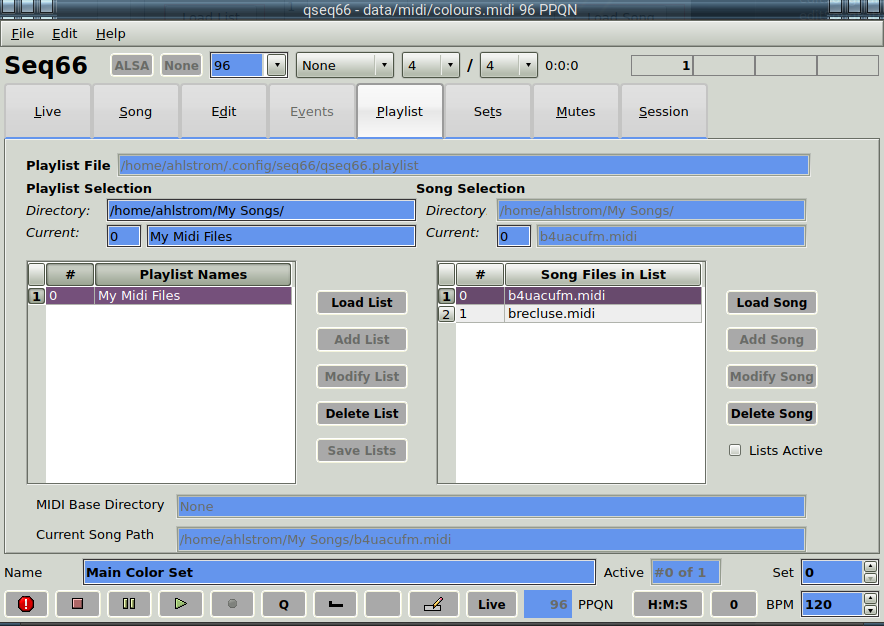
\includegraphics[scale=0.75]{main-window/main-window-stylesheet.png}
   \caption{Seq66 View with Style Sheet Applied}
   \label{fig:view_with_style_sheet_applied}
\end{figure}

\paragraph{'usr' File / Additional Options / [user-session]}
\label{paragraph:user_file_added_options_session}

   \texttt{[user-session]} provides a way to cooperate with the
   \textsl{Non Session Manager}.

   \begin{verbatim}
   [user-session]
   session = none
   url = ""
   \end{verbatim}

   See \sectionref{subsec:sessions_nsm_before_using_nsm}; it goes into great
   detail.

\paragraph{'usr' File / Additional Options / [new-pattern-editor]}
\label{paragraph:user_file_added_options_pattern_editor}

   \texttt{[new-pattern-editor]} contains settings values for recording
	 when a new pattern editor is opened. A new pattern is indicated when
	the loop has the default name, \textsl{Unititled}.
 	These values save time during a live recording session.
   The valid values for record-style are \texttt{merge},
 	\texttt{overwrite}, and \texttt{expand}.

   \begin{verbatim}
   [new-pattern-editor]
	armed = false
	thru = false
	record = false
	qrecord = false
	record-style = merge
   \end{verbatim}

\subsection{'ctrl' File}
\label{subsec:configuration_ctrl}

   Like \textsl{Seq24}, \textsl{Seq66} provides a way to control the
   application to some extent via a MIDI controller, such as a MIDI keyboard or
   a MIDI pad device.  The current section describes this feature;
   additional resources and ideas can be found at \url{linuxaudio.org}
   (\cite{midicontrol}).
   Also see the tutorial section \sectionref{sec:launchpad_mini}.
   An \textsl{Open Document Format} spreadsheet shows layouts for the default
   keystroke configuration (including pattern, mutes, and automation controls)
   and for a couple of \textsl{Launchpad Mini} configurations.

   The 'ctrl; file provides settings for keyboard control, MIDI control, and for
   specifying MIDI output to reflect \textsl{automation} commands in a device
   such as the \textsl{LaunchPad}..
   The name of this file is specfied in the 'rc' file as noted earlier.

\subsubsection{'ctrl' File / MIDI Control Settings}
\label{subsubsec:configuration_ctrl_midi_control_settings}

   \begin{verbatim}
      /home/user/.config/seq66/qseq66.usr
   \end{verbatim}

   This file offloads the control settings from the 'rc' file, for a more
   flexible setup. It starts with the sections common to all \textsl{Seq66}
   configuration files.  The first unique section defines some useful settings
   using the new variables feature of the configuration.  Look at the sample or
   generated file to see the layout of these items.

   \begin{itemize}
      \item \texttt{load-key-controls}.
         Generally, this should always be set to "true".
      \item \texttt{load-midi-controls}.
         This one could plausibly disabled, but for live performance will
         certainly be set to "true".
      \item \texttt{control-buss}.
         The control-buss value ranges from 0 to the maximum buss provided by
         the hardware on the system. If set, then only that buss will be allowed
         to send MIDI control.  A value of 255 or 0xff means any buss can send
         MIDI control.
      \item \texttt{midi-enabled}.
         If set to "true", then the MIDI controls will be used.
         It can be set to "false", while keeping the configuration in place
         for later usage.
      \item \texttt{button-offset}.
         This item provides a way to move a set of input controls (e.g. from a
         \textsl{Launchpad Mini}) to a different area of the input control
         device.  Not yet supported.
      \item \texttt{button-rows}.
         Indicates the rows of the input control grid.
         Still in progress.
      \item \texttt{button-columns}.
         Indicates the columns of the input control grid.
         Still in progress.
   \end{itemize}

\subsubsection{'ctrl' File / Loop Control}
\label{subsubsec:configuration_ctrl_loop_control}

   The loop-control group consists of 32 lines (0 to 31), one for each
   pattern slot shown in the patterns panel.
   It provides a way to control the arming/disarming (muting/unmuting) of
   each pattern shown in the patterns panel.
   It consolidates the keyboard and MIDI control settings into one table.

   Note that the main window shows the \textsl{active} screen-set.
   These MIDI controls affect the \textsl{active} screen-set.

   This block of matrix elements, numbered from 0 to 31,
   represent control functions (toggle, mute, unmute) for the 32 patterns
   of the active screen-set.
   These 32 rows correspond to the hot-keys assigned in
   the \textbf{File / Options / Keyboard / Control keys [keyboard-group]} 
   configuration panel.

   \index{[loop-control]}
   The MIDI control section begins with the following "INI"-style
   group marker tag, followed by one stanza-line per loop:

   \begin{verbatim}
      [loop-control]
      # Control:  Toggle          On               Off
      0 "1" [ 0 0x00 0 0 0 ] [ 0 0x00 0 0 0 ] [ 0 0x00 0 0 0 ]  # Loop 0
      . . .
   \end{verbatim}

   The first number is an index number, starting at 0.  It indicates what
   loop the control line will affect.
   The numbers in the leftmost brackets define a \textsl{Toggle} control;
   the numbers in the middle brackets define an \textsl{On} control;
   the numbers in the rightmost brackets define an \textsl{Off} control.
   The numbers inside each set of brackets define six values that set up the
   control.  The layout of each filter inside the brackets is as follows:

      \textbf{[INV STAT D1 D2min D2max]}

   \begin{itemize}
      \item \textbf{INV} = \textbf{inverse}
      \item \textbf{STAT} = \textbf{MIDI status byte} (channel included) 
      \item \textbf{D1} = \textbf{data1}
      \item \textbf{D2min} = \textbf{data2 min}
      \item \textbf{D2max} = \textbf{data2 max}
   \end{itemize}

   If \textbf{STAT} is not 0x00, the control is enabled.  \textsl{Seq66} will
   match the incoming MIDI event against the \textbf{STAT (MIDI status byte)}
   pattern (e.g. a Note On event), and perform the action (On/Off/Toggle) if
   the \textbf{D1} (e.g. a Note number), matches the incoming data, and the
   incoming parameters (e.g. Note velocity) falls in the specified
   \textbf{D2min} to \textbf{D2max} range.  All data values are best specified
   in decimal.

   The \textbf{INV (inverse)} field will make the pattern perform the opposite
   action (\textsl{off} for \textsl{on}, \textsl{on} for \textsl{off}) if the
   data falls outside the specified range.  This is cool because one can map
   several sequences to a knob or fader.

   The \textbf{STAT (MIDI status byte)} field is a MIDI status byte number in
   decimal or hexadecimal notation.
   Remember that it can include a channel.  This channel is not overridden by
   the pattern's selected channel when a MIDI control matching event is
   received. 
%  The channel nybble of this byte is ignored.
   One can look up the possible status values up in the MIDI messages tables;
   the relevant data can be found at \cite{midicontroltable}.
%  As the channel on which the events are sent is ignored,
%  it is sufficient to use the values for channel 1; that is, 0.

   The last three fields describe the range of data that will match.  The
   \textbf{D1 (data1)} field provides the actual MIDI event message number to
   detect, in decimal.  This item could be a Note On/Off event or a
   Control/Mode change event, for example.

   The \textbf{D2min (data2 min)} field is the minimum value of the event for
   the filter to match. For Note On/Off events, this would be the velocity
   value, for example.

   The \textbf{D2max (data2 max)} field is the maximum value of the event for
   the filter to match.

%  This set of values is explained below.

   For each pattern, we can set up MIDI events to turn a 
   pattern on, off, or to toggle it.

   The MIDI control setup resembles a matrix.  This matrix is divided into a
   number of sections depending on the overall functionality of the MIDI
   controls in the section:

\subsubsection{'ctrl' File / Mute-Group Control}
\label{subsubsec:configuration_ctrl_mute_group_control}

   \index{mute-group control}
   This section provides controls for 32 groups of mutes.
   A group is a set of patterns that can toggle their playing state
   together.  Every group contains all 32 sequences in the active screen set.
   So, this part of the MIDI Control section is used for muting and unmuting
   (and toggling) a group of patterns using a keystroke or MIDI control.
   The definitions are in the same format as the loop-control section.

   \begin{verbatim}
      [mute-group-control]
       0 "!" [ 0 0x00 0 0 0 ] [ 0 0x00 0 0 0 ] [ 0 0x00 0 0 0 ]  # Mute 0
       . . .
   \end{verbatim}

   All this section does is set up the controls to be used; the actual
   mute-group patters are defined in a 'mutes' configuration file.

\subsubsection{'ctrl' File / Automation Control}
\label{subsubsec:configuration_midi_ctrl_automation}

   This section provides ways to control \textsl{Seq66} push-button controls
   from a keyboard or from a MIDI device.
   These entries control
   \textsl{Seq66} actions like changing the BPM value, screen-set,
   record, solo, etc.
   
   Each item in this group consists of one line.  Each line
   specifies a MIDI event that can cause a given
   \textsl{Seq66} user-interface operation to occur.
   These items are easy to view in the 'ctrl' configuration file,
   in the \texttt{[automation-control]} section.

   \begin{verbatim}
      [automation-control]
       0 "'" [ 0 0x00 0 0 0 ] [ 0 0x00 0 0 0 ] [ 0 0x00 0 0 0 ]  # BPM Up
       . . .
   \end{verbatim}

   The stanzas meaning can change depending on the type of control.  Here are
   the important styles:

   \begin{verbatim}
      Normal:        [ Toggle       ] [ On          ] [ Off             ]
      Playback:      [ Pause Play   ] [ Start Play  ] [ Stop Play       ]
      Play list:     [ Select by D2 ] [ Select Next ] [ Select Previous ]
      Play song:     [ Select by D2 ] [ Select Next ] [ Select Previous ]
   \end{verbatim}

   For selecting play-lists and songs by number, \textbf{D2} is used.
   Thus, one possible value to use to select would be to use a 
   Note On event on channel 16 (0x9F) with a note number of 0 (a rarely-used
   note in any tune), and list/song numbers ranging from 0 to 127.  Using note
   0 for list selection and note 1 for song selection:

   \begin{verbatim}
      24 "F2" [ 0 0x9F   0   0 127 ] [ . . . ] [ . . .] # Play List
      25 "F3" [ 0 0x9F   1   0 127 ] [ . . . ] [ . . .] # Play Song
   \end{verbatim}

   Obviously, this requires a MIDI controller for which the velocity can be
   exactly specified.  One can also reserve \textbf{D2} values of 126 for
   "previous" and 127 for "next".

\paragraph{Automation / BPM Up and Down}
\label{paragraph:configuration_midi_ctrl_bpmupdn}

   These controls increment or decrement the beats-per-minute setting, as if
   the up- or down-arrow has been clicked in the BPM combox-box, or the up- or
   down-arrow key pressed, in that combo-box.
   This increment is the
   \index{bpm!step increment}
   \index{usr!step increment}
   "step increment" which defaults to 1, but can be modified by
   changing the "bpm\_step\_increment" value in the 'usr'
   configuration file.

\paragraph{Automation / Screen-Set Up and Down}
\label{paragraph:configuration_midi_ctrl_ssupdn}

   Also abbreviated "Set Up" and "Set Down".
   This control increments / decrements to the next / previous screen-set. 
   Once the screen-set has been altered, mute-groups and other
   actions apply to that screen set.

\paragraph{Automation / Mod Replace}
\label{paragraph:configuration_midi_ctrl_modrep}

   This control the "replace" flag.
   Then, when the user manually clicks a pattern slot,
   that pattern is unmuted, and all the rest are muted.
   Thus, this MIDI control is kind a of "Solo" function.
   It works whether in "Live" or "Song" mode.

\paragraph{Automation / Mod Snaphot}
\label{paragraph:configuration_midi_ctrl_modsnap}

   This control causes the playing statuses of all active
   (i.e. having data) patterns to be saved.  When turned off, the
   original playing status is restored.  Thus, two MIDI events
   need to be allocated to this functionality.

\paragraph{Automation / Mod Queue}
\label{paragraph:configuration_midi_ctrl_modqueue}

   This control sets up the "queue" status flag.
   Then, when the user manually clicks a pattern slot,
   that pattern is queued, and will play at the next cycle of the
   pattern.

   Here is an example from \cite{midicontrol}, which shows how to set up
   the "Sustain" control-change event to queue or un-queue a sequence:
   The \textsl{Akai MPK Mini} has a Sustain button and we can set the
   Sustain MIDI event (with MIDI status byte 176 [0xB0] to represent a
   Controller event, and control/mode change number 64 [0x40] to
   represent the Sustain or Pedal control) up as the queue modifier in
   the \texttt{mod queue} entry:

   \begin{verbatim}
      6 "o" [ 0  0x00 0  0  0 ] [ 0  0xB0 64 127 127 ] [ 0  0xB0 64 0  0 ]
      #      INV STA  D1 mn mx   INV STA  D1 mn  mx     INV STA D1  mn mx
      #                                   ^  ^                      ^  ^
      #                                   |  |                      |  |
      #                                   |   ----Sustain-----------   |
      #                                    -------Control Change-------
   \end{verbatim}

   So when the Sustain button is held down, and one presses one of the pads
   on the \textsl{MPK Mini}, the corresponding sequence gets queued.

   Also include in the data directory are sample 'ctrl' files for other devices.

\paragraph{Automation / Mute Group}
\label{paragraph:configuration_midi_ctrl_modgmute}

   This MIDI control sets up a "group learn".
   This control sets two internal flags on : "mode-group" and "group-learn".
   The first flag indicates that we will be handling mute-groups.
   The second flag indicates that we are learning these mute-groups,
   effectively recording the current status of all the patterns in all of the
   screen-sets.

   \index{L button}
   Note that this control corresponds to the "L" button in the main window
   user-interface.
   \index{keys!l}
   It can also be accessed by the default hot-key, \texttt{l}.

   Note that, once in learn-mode, there is no way to cancel learn-mode
   except by selecting an illegal mute-group keystroke.
   Also see \sectionref{sec:mutes_master}.

\paragraph{Automation / Screen-Set Play}
\label{paragraph:configuration_midi_ctrl_ssplay}

This MIDI control sets the playing screen-set.

\subsubsection{Automation / More MIDI Control}
\label{subsubsec:configuration_midi_ctrl_automationex}

   Many additional control items were requested by users, to control
   additional features of the application.  Too many to list here.
   See the 'ctrl' file samples for more information.

\subsubsection{'ctrl' File / MIDI Control Output}
\label{subsubsec:configuration_ctrl_midi_control_out}

   This section provides a way to have a MIDI device, such as the
   \textsl{Novation Launchpad Mini}, show the status
   of the patterns that are active, as well as other information.

   \begin{verbatim}
      [midi-control-out-settings]
      set-size = 32
      output-buss = 1
      enabled = false
      button-offset = 0
      button-rows = 8
      button-columns = 8
   \end{verbatim}

   The first section sets up some general settings.

   \begin{itemize}
      \item \texttt{set-size}.
         Provides the set size.  The default is 32, in a 4 x 8 grid.
      \item \texttt{output-buss}.
         Indicates where automation-display controls are to be sent.
         Specify the output buss to which the display device is attached.
      \item \texttt{midi-enabled}.
         If set to "true", then the MIDI control outputs will be used.
         It can be set to "false", while keeping the configuration in place
         for later usage.
      \item \texttt{button-offset}.
         This item provides a way to move a set of output controls (e.g. from a
         \textsl{Launchpad Mini}) to a different area of the output control
         device.  Not yet supported.
      \item \texttt{button-rows}.
         Indicates the rows of the output control grid.
         Still in progress.
      \item \texttt{button-columns}.
         Indicates the columns of the output control grid.
         Still in progress.
   \end{itemize}

   \begin{verbatim}
      [midi-control-out]
      0 [1  0 0x90   0 60] [1  0 0x90   0 15] [1  0 0x90   0 62] [1  0 0x90   0 12]
      . . .
   \end{verbatim}

   The first number is the pattern number of the pattern whose armed/muted
   status is to be shown.
   There are samples in the \texttt{data/linux} directory for some devices that
   one can adapt to other equipment.

   There are additional automation controls whose status can be displayed:

   \begin{verbatim}
      # MIDI Control Out: play on/off
      0 [ 0x0 0 0 ] [ 0x0 0 0 ]
      # MIDI Control Out: stop on/off
      0 [ 0x0 0 0 ] [ 0x0 0 0 ]
      # MIDI Control Out: pause on/off
      0 [ 0x0 0 0 ] [ 0x0 0 0 ]
      # MIDI Control Out: queue on/off
      0 [ 0x0 0 0 ] [ 0x0 0 0 ]
      # MIDI Control Out: oneshot on/off
      0 [ 0x0 0 0 ] [ 0x0 0 0 ]
      # MIDI Control Out: replace on/off
      0 [ 0x0 0 0 ] [ 0x0 0 0 ]
      # MIDI Control Out: snap store/restore
      0 [ 0x0 0 0 ] [ 0x0 0 0 ]
      # MIDI Control Out: reserved
      0 [ 0x0 0 0 ] [ 0x0 0 0 ]
      # MIDI Control Out: learn on/off
      0 [ 0x0 0 0 ] [ 0x0 0 0 ]
   \end{verbatim}

   See the sample files for more detailed descriptions.

\subsection{'mutes' File}
\label{subsubsec:configuration_mute_group_control}

   This file starts with:

   \begin{verbatim}
      [mute-group-flags]
      save-mutes-to = both
      mute-group-rows = 4
      mute-group-columns = 8
      mute-group-selected = -1
      groups-format = bin
   \end{verbatim}

   These variables are described in the sample 'mutes' file.
   The mute-in group consists of 32 lines (32 to 63), one for each
   pattern box.
   It provides a way to control the mute groups.
   A group is a set of sequences that can arm their playing state
   together; every group contains all 32 sequences in the
   \textsl{active} screen-set.

   This section is delimited by the \texttt{[mute-group]} construct.
   It controls 32 groups of mutes in the same way as defined for
   \texttt{[midi-control]}. A group is set of sequences that can toggle their
   playing state together.  Every group contains all 32 sequences in the
   active screen set.

   \begin{verbatim}
      [mute-groups]
       0 [ 0 0 0 0 0 0 0 0 ] [ 0 0 0 0 0 0 0 0 ] [ . . .] [ 0 0 0 0 0 0 0 0 ]
       1 [ 0 0 0 0 0 0 0 0 ] [ 0 0 0 0 0 0 0 0 ] [ . . .] [ 0 0 0 0 0 0 0 0 ]
       . . .
      31 [ 0 0 0 0 0 0 0 0 ] [ 0 0 0 0 0 0 0 0 ] [ . . .] [ 0 0 0 0 0 0 0 0 ]
   \end{verbatim}

   In this group are the definitions of the state of the 32 (or more, once the
   support for larger sets is completely worked out) sequences
   in the playing screen set when a group is selected.
   Each set of brackets defines a group.
%  After the list of sequences and their MIDI events, one can 
%  set \textsl{Seq66} to handle MIDI events and change some more settings
%  in \texttt{seq66.rc}.
%
%  What is the different between the \textbf{mute-in group}
%  section and the \textbf{mute group} section?  The former defines the MIDI
%  control values that can affect the muting of a group, while the latter
%  specifies the patterns that are part of a group.

\subsection{'drums' File}
\label{subsec:configuration_drums}

   The 'drums' file is based on a similar file created using the \texttt{midicvt}
   application (also available on \textsl{GitHub}.
   This file is also referred to as the 'note-mapper' file.

   \begin{verbatim}
      [notemap-flags]
      map-type = drums
      gm-channel = 10
      reverse = false
   \end{verbatim}

   These settings are explained in the sample 'drums' files.  In addition, the file
   includes a number of sections that define the number and name of the
   original "drum", and the \textsl{General MIDI} device to which it corresponds.

   \begin{verbatim}
      [Drum 36]
      dev-name = "Bass Drum Gated Reverb"
      gm-name = "Bass Drum 1"
      dev-note = 36
      gm-note = 36
   \end{verbatim}

   This file is useful mainly when obtaining drum tracks recorded with devices in
   the early days of MIDI, where each vendor provided their own peculiar layout of
   percussion sounds.

\subsection{'palette' File}
\label{subsec:configuration_palette}

   This file is described in the chapter on palettes, \sectionref{sec:palettes}.

\subsection{'playlist' File}
\label{subsec:configuration_playlist}

   This file is described in the chapter on playlists, \sectionref{sec:playlist}.

%-------------------------------------------------------------------------------
% vim: ts=3 sw=3 et ft=tex
%-------------------------------------------------------------------------------
